%Präambel
\documentclass[paper=a4,fontsize=11pt,headsepline,footsepline,parskip=half]{scrartcl}
\usepackage[utf8]{inputenc}
\usepackage[T1]{fontenc}
\usepackage{amsmath,amsfonts,amssymb}
\usepackage{ngerman,graphicx,textcomp,mathpazo,booktabs}
\usepackage[decimalsymbol=comma,per=frac]{siunitx}
\usepackage[textfont=sl,labelfont=bf]{caption}

%Seite einrichten
\areaset[2cm]		% Zusätzlicher Rand für die Bindung
        {17cm}{24cm}	% Textbreite und -Höhe

%Zeilenabstand
\linespread{1.2} %Standardwert

%Kopf- und Fußzeile
\usepackage{scrlayer-scrpage}
\setlength{\headheight}{23pt}
\lohead{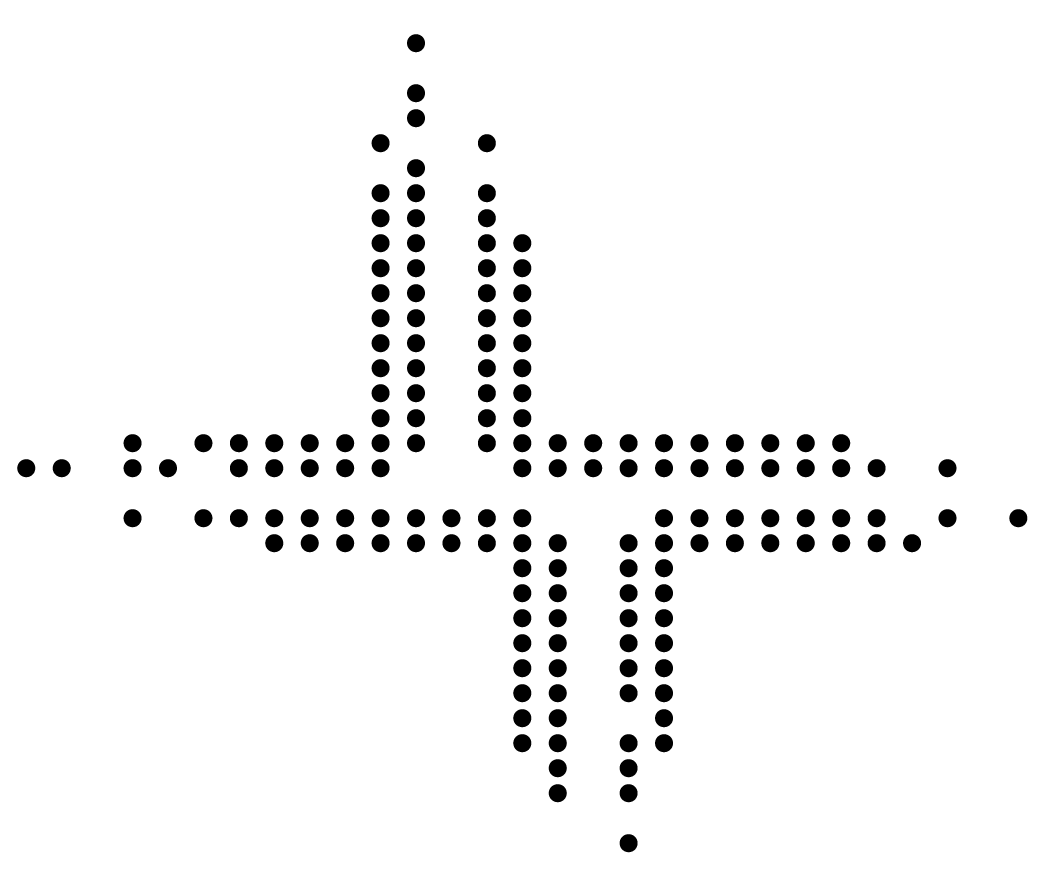
\includegraphics[width=0.7cm]{../logofbi} Hochschule Darmstadt}
\rohead{David Falk, Christian Lichtsinn}
\pagestyle{scrheadings}

%Programmierzeilen
\usepackage{listings}
%Optionen für listings
\lstset{
frame=single, %Rahmen
numbers=left %Zeilennummer
}

%sollte als letztes Paket geladen werden
\usepackage{hyperref}

\begin{document}

%Titelblatt
\begin{titlepage}

\begin{minipage}[c]{5cm}
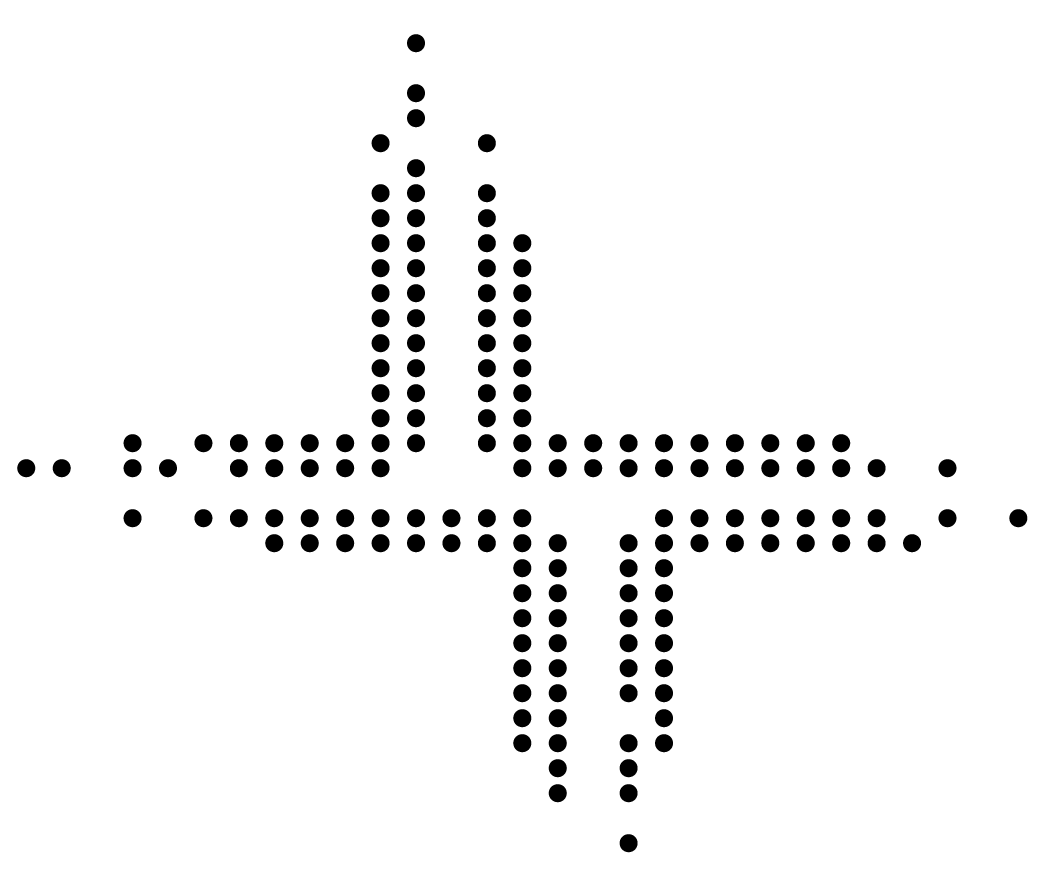
\includegraphics[width=5cm]{../logofbi}
\end{minipage}
\hfill
\begin{minipage}[c]{10cm}
\begin{flushright}
\Large Einführung in die Technik\\und Anwendung von\\
\LARGE \textbf{RFID}
\end{flushright}
\end{minipage}

\vspace*{1cm}

\begin{minipage}[c]{9cm}
\begin{flushleft}
\large David Falk (736532)\\Christian Lichtsinn (736787)\\Praktikum 4: 30.11.15: \textbf{Mo-56x}
\end{flushleft}
\end{minipage}
\hfill
\begin{minipage}[c]{7cm}
\begin{flushright}
\large Betreuer:\\Prof. Ralf S. Mayer\\F. Dotzauer
\end{flushright}
\end{minipage}

\vspace*{1cm}

%Workaround nötig wegen parskip Option.
\begingroup
  \setlength{\parskip}{0pt}% keinen Absatzabstand einfügen
  \setlength{\parindent}{0pt}% nicht einziehen
  \setlength{\parfillskip}{0pt plus 1fil}% Absatz darf komplett gefüllt sein
  \par\rule{\linewidth}{1.5pt}\par
\endgroup

\vspace*{\stretch{1}} %stretch zählt all stretch zusammen (hier 1+2=3) und verteilt den vspace entsprechend, hier 1/3

\centering
\Huge{\textbf{\textsl{HF- und UHF-Leser\\Setup \& Tests}}}

\vspace*{\stretch{2}} %und hier 2/3 vspace vom Rest der Seite.

\end{titlepage}

%KAPITEL 1
\section{Fragen zu HF scemtec}

\subsection{In welchem Frequenzband arbeitet ISO 15693?}

Bei $13,56 MHz$, HF (high frequency).

\subsection{Was versteht man unter STX und ETX bei der seriellen Übertragung zum Gerät?}

STX und ETX sind so etwas wie Funktionsklammern. Sie stehen für \textbf{Start of Transmission} (STX) und \textbf{End of Transmission} und
umschließen einen Funktionsaufruf. Beispiel:

\begin{lstlisting}
 STX "F000" <vv> ETX {c}
\end{lstlisting}

\subsection{Was muss man bei der Zusammensetzung eines Kommandos über serielle Schnittstelle an den scemtec-Reader beachten?}

Die Prüfsumme hinter dem Kommando muss stimmen (siehe Code oben, das \textbf{\{c\}}).

%KAPITEL 2
\section{Fragen zu SamSys-UHF-Reader}

\subsection{Wie ist das Lesegerät MP9320 in Betrieb zu nehmen, was ist zu beachten, wie wird die Antenne angeschlossen?}

Das Lesegerät verbindet man mit einem seriellem Kabel mit einem PC, damit man via einer Software mit dem Lesegerät kommunizieren kann. Das MP9320
darf dabei aber erst in Betrieb genommen werden, wenn entweder an den Antennenanschlüssen entsprechende UHF-RFID-Antennen angeschlossen sind oder
sich ein $50\ohm$-Abschlusswiderstand anstatt der Antenne befindet. Die Antennen werden der Reihe nach zuerst an Anschluss 1 und so weiter angeschlossen.

\subsection{Könnten mehrere UHF-Lesegeräte sich gegenseitig beeinflussen?}

Ja, es wird aber versucht dies durch Anti-Kollisionsverfahren zu vermeiden.

\subsection{Was bedeutet ISO 18000-6?}

ISO 18000-6 ist eine Norm für die Spezifikation der Luftschnittstelle im UHF-Bereich (Ultra High Frequency) von $860 MHz$ bis $960 MHz$.

\subsection{Wie können Tags mit der RF Command Suite und der RS232-Schnittstelle gelesen werden?}

Sofern im Reiter \textbf{RFCS Config} ein Haken bei \textbf{Parse Received Data} gesetzt ist, kann man im Reiter \textbf{Tag Summary} Tags
automatisch einlesen, sofern sie sich im Empfangsbereich der Antenne befindet. Alternativ kann man im Reiter \textbf{Command} Tags mit dem Befehl
\textbf{\}Rd!} auslesen.

%KAPITEL 3
\section{scemtec}

\subsection{Reichweite und Leserate}

Bei unseren Tests bezüglich der Reichweite sind wir mit den Tags erstmal so weit wie möglich von der Antenne weg und haben uns dieser dann langsam
genähert, bis das Programm Unidemo angezeigt hat, dass es einen der Tags gefunden hat. Die geschätzte Reichweite beträgt 1 bis 2 Meter.

Um die Leserate zu bestimmen, haben wir 10 Tags an der Antenne platziert und diese via Unidemo 60 Sekunden lang auslesen lassen. Dabei ergab sich eine
durchschnittliche Leserate von 18,3 Reads/s.

\subsection{Unidemo-Kommandos}

Beim Scannen der Tags setzt die Unidemo-Software folgende Befehle ab:

\begin{lstlisting}
 [STX]6a20s[ETX]!
 [STX]6b20s[ETX]$
 [STX]6c20s[ETX]%
 [STX]6aa0s[ETX]t
 [STX]6ab0s[ETX]w
\end{lstlisting}

Wichtig dabei sind die 4 Ziffern nach [STX], also 6a20, 6b20 und so weiter. Diese sind jeweils High-Level-Funktionen zum Erkennen von Tags,
die verschiedenen Standards folgen. Diese sind in diesem Falle \textbf{ICode 1} (6a20), \textbf{Tag-it} (6b20), \textbf{ISO 15693} (6c20) und
\textbf{ICode EPC/UID} (6aa0/6ab0). Aus der Antwort konnten wir herauslesen, dass nur für \textbf{ISO 15693} Tags gefunden wurden.

\subsection{STX/ETX-Befehle und Antworten}

Im vorherigen Unterkapitel haben wir bereits herausgefunden, dass wir Tags nach ISO 15693 für den Versuch zur Verfügung haben. Um diese Tags zu
finden und die Anzahl der Tags auszumachen, geben wir folgenden Befehl ein und erhalten diese Antwort:

\begin{lstlisting}
 [STX]6c20s[ETX]%
 [ACK][STX]6c20000008[ETX]
\end{lstlisting}

Dabei bedeutet die Antwort:

$[ACK][STX]\underbrace{6c20}_{\text{Befehl}}\underbrace{00}_{\text{OK}}\underbrace{0008}_{\text{Anzahl der gefundenen Tags}}[ETX]$

Um nun die IDs eines oder mehrerer Tags auszulesen, benötigt man folgenden Befehl (wir haben vergessen die Prüfsumme zu notieren, daher nur ein ?):

\begin{lstlisting}
 [STX]6c21[ETX]?
 [ACK][STX]6c210001133DC34C000104E0[ETX]
\end{lstlisting}

Dabei bedeutet die Antwort:

$[ACK][STX]\underbrace{6c21}_{\text{Befehl}}\underbrace{0001}_{\text{Anzahl Tags}}\underbrace{13}_{\text{DSFID}}\underbrace{3DC34C000104E0}_{\text{ID 64bit in umgekehrter Byte-Reihenfolge}}[ETX]$

DSFID bedeutet Data Storage Format Identifier. Wenn mehrere Tags gefunden werden, werden die IDs jeweils hintereinander aufgeführt.

Mit Kenntnis der ID des Tags kann man den Tag selbst auslesen. Leider ist uns hier ein Fehler unterlaufen. Wir dachten, dass schon der vorherige
Schritt den Inhalt des Tags ausliest, da dieser in der Dokumentation \textbf{Get Inventory} genannt wird, was wir für das Auslesen der Blöcke hielten.
Was wir hätten nutzen sollen wäre die Funktion \textbf{4C20} für \textbf{Advanced Read Single Block} oder \textbf{4C24} für \textbf{Advanced Read Multiple Blocks}.
Für beide Befehle benötigt man die ID des Tags, die wir mit dem Befehl weiter oben auslesen konnten.

\section{SamSys}

\subsection{Messreihe}

In dieser Messreihe wurde nach und nach ein weitere Tag in den Empfangsbereich der UHF-Antenne gelegt und geschaut, ob die Tags alle erkannt wurden
und wie oft sie erkannt wurden (und damit die Leserate). Dabei wurde der Testzeitraum auf 10 Sekunden gesetzt und via der RF Command Suite
ausgewertet. Die Software ist in der Lage die Tags zu unterscheiden und anzuzeigen, wie oft diese innerhalb der 10 Sekunden erkannt wurden.

\begin{center}
\begin{tabular}{@{}cccc@{}}
\toprule
\multicolumn{3}{r}{Reads / s}\\
\cmidrule(lr){2-4}
  Anzahl Tags & 1. Messreihe & 2. Messreihe & 3. Messreihe\\
\midrule
 1 & 237 & 60 & 17\\
 2 & 96, 99 & 1, 3 & 16, 24\\
 3 & 8, 9, 3 & 15, 8, 19 & 9, 9, 14\\
 4 & 16, 6, 13, ? & 24, 22, 25, ? & 32, 33, 34, ?\\
 5 & 14, 30, 31, 31, ? & 2, 5, 4, 7, ? & 40, 39, 45, 40, 42\\
\bottomrule
\end{tabular}
\captionof{table}{\label{tab:messreihe}Messwerte für ansteigende Anzahl an Tags im Empfangsbereich der UHF-Antenne. ? bedeutet hier, dass der
Tag nicht erkannt wurde. Angegeben werden die Reads/s für jedes einzelne Tag.}
\end{center}

\begin{center}
 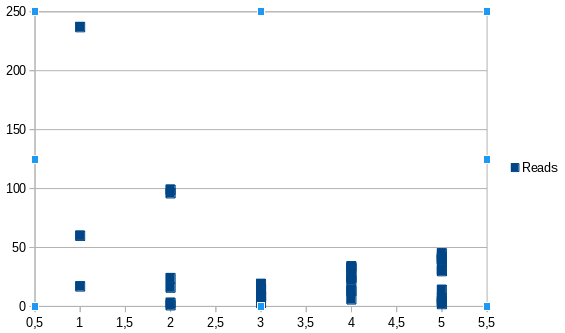
\includegraphics[width=0.7\linewidth]{messreihe}
 \captionof{figure}{\label{fig:messreihe}Messwerte aus Tabelle \ref{tab:messreihe} in Diagrammform.}
\end{center}

Wie man an den Messreihen sehen kann, gibt es viele Ausreißer, vor allem wenn wenige Tags vorhanden sind. Die Frage ist hier aber, wie aussagekräftig
die Daten sind, da sich die UHF-Geräte gegenseitig stark beeinflussen. Es gibt zwar Anti-Kollisionsverfahren, aber je mehr Anti-Kollision betrieben
werden muss, umso stärker sollte die Leserate runtergehen. Wie groß dieser Einfluss ist, müsste man aber mit weiteren Messreihen feststellen, für
die leider keine Zeit im Praktikum war.

Was man ableiten kann ist, dass wenn die Lesegeräte ungestört sind, ist die Leserate beträchtlich (siehe Tabelle \ref{tab:messreihe} auf Seite
\pageref{tab:messreihe}, 1. Messreihe für einen Tag) und mit zunehmender Anzahl wird es schwerer, alle Tags zu erkennen.

\subsection{Ansteuerung via Terminal}

Das SamSys lässt sich auch via Terminalprogramm ansteuern. Der Befehl \textbf{\}Rv!} gibt die Version aus. \textbf{\}Cr!} gibt die Register aus und
mit \textbf{\}Rd!} kann man Tags auslesen.

\end{document}
